\documentclass[11pt]{article}
\usepackage[utf8]{inputenc}
\usepackage[T1]{fontenc}
\usepackage{amsmath,amssymb,amsfonts,amsthm}
\usepackage{graphicx}
\usepackage{booktabs}
\usepackage[numbers,sort&compress]{natbib}
\usepackage{xcolor}
\usepackage{enumitem}
\usepackage{caption}
\usepackage{placeins}
\usepackage[margin=2.5cm]{geometry}
\usepackage{fancyhdr}
\usepackage{hyperref}
\hypersetup{hidelinks}
\newtheorem{proposition}{Proposition}
\newtheorem{remark}{Remark}
\pagestyle{fancy}
\fancyhead[L]{\small Preprint. Under review.}
\fancyhead[R]{}\fancyfoot[C]{\thepage}
\renewcommand{\headrulewidth}{0pt}

\title{\textbf{Psychometric Content Routing:}\\
\Large Frontier-Value Selection for\\User-Conditioned LLM Processing}
\author{Jung Min Kang\thanks{Email: \texttt{gangjeongmin23@gmail.com}}\\
Independent Researcher\\
Seoul, South Korea}
\date{May 2026}

\begin{document}
\maketitle\thispagestyle{fancy}

\begin{abstract}
When a large language model must select which content to process under a fixed token budget, standard approaches either treat all content uniformly or select by difficulty alone.
We propose \textbf{Psychometric Content Routing~(PCR)}, a framework grounded in Item Response Theory (IRT; Lord \& Novick, 1968) and the Linear Logistic Test Model (LLTM; Fischer, 1973).
The \emph{Frontier Value Function} $\mathcal{F}(\theta,b) = P(1{-}P)$ peaks when user ability $\theta$ matches content difficulty $b$, providing a principled selection signal.
We validate PCR on Llama~3.3~70B (via Groq) across 20 real science passages at five difficulty levels with six user profiles, routing on author-assigned difficulty labels validated by LLM rating ($\rho = 0.919$).
Under equal token budgets, PCR strongly outperforms difficulty-only routing ($6.06 \pm 1.39$ vs.\ $3.67 \pm 2.36$; Cohen's $d = 1.23$; pairwise win rate 83\%, $p = 0.004$) and trends above corpus-prefix and random selection.
LLTM hand-crafted features provide a weaker but API-free difficulty proxy ($\rho = 0.50$), offering a scalable path when LLM-based rating is unavailable.
To our knowledge, PCR is among the first explicit uses of IRT ability--difficulty interaction for user-conditioned content routing at inference time.
\end{abstract}

\section{Introduction}

Large language models process content uniformly regardless of who consumes the output.
Under token constraints, \emph{which chunks deserve deep processing for this user?} becomes critical.
Existing methods select by relevance or difficulty without user conditioning.

Psychometrics formalized both ingredients: IRT~\citep{lord1968statistical} separates ability $\theta$ from difficulty $b$; LLTM~\citep{fischer1973lltm} decomposes difficulty into features.
In adaptive computation, Mixture-of-Depths~\citep{raposo2024mod} and GateSkip~\citep{laitenberger2025gateskip} skip layers for easy tokens without user conditioning.
Concurrently, Yang et al.~\citep{yang2026zpd} proposed ZPD Detector, using IRT-based capability--difficulty matching for training data selection.
PCR differs in applying the frontier-value signal to user-facing content routing at inference time.

\paragraph{Contributions.}
(1)~PCR: IRT-based user-conditioned content selection at inference time.
(2)~Frontier Value Function with water-filling characterization.
(3)~Real-LLM validation: $d = 1.23$, $p = 0.004$, 83\% pairwise win rate.
(4)~LLTM evaluated as a scalable API-free difficulty proxy ($\rho = 0.50$).

\section{Method}

\subsection{Frontier Value Function}

\begin{equation}
\mathcal{F}(\theta,b) = P(1-P), \quad P = \sigma(a(\theta - b))
\end{equation}

$\mathcal{F}$ peaks at $\theta = b$---the user's frontier~\citep{vygotsky1978mind}---and vanishes at both extremes (Figure~\ref{fig:fv}).

\begin{figure}[htbp]
\centering
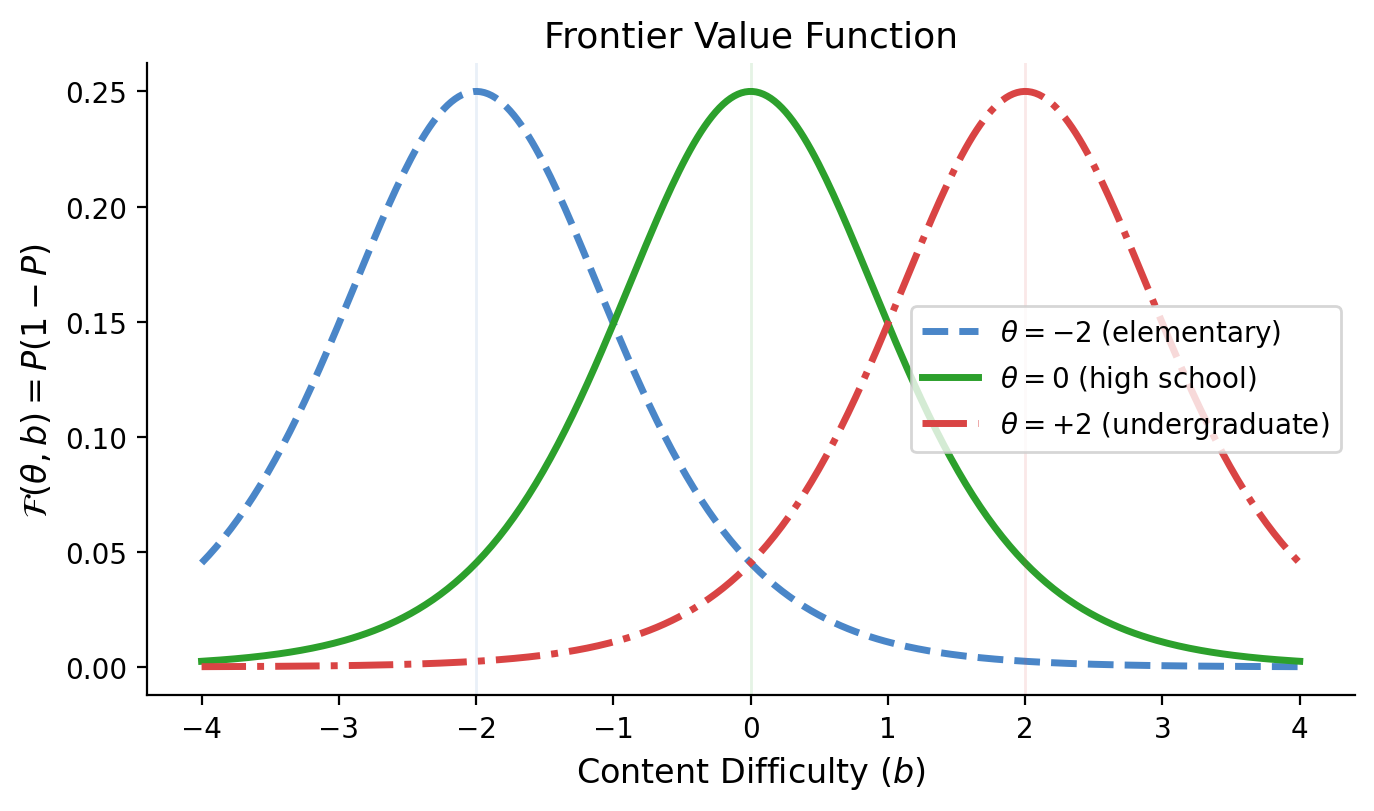
\includegraphics[width=0.65\linewidth]{figures/fig1_frontier_value.png}
\caption{Frontier Value $\mathcal{F}(\theta,b)$ for three ability levels.}
\label{fig:fv}
\end{figure}

\begin{remark}[Fisher information]
$\mathcal{I} = a^2 P(1{-}P) = a^2 \mathcal{F}$.
We use $\mathcal{F}$ to avoid disproportionate weighting by high-discrimination items.
\end{remark}

\FloatBarrier

\subsection{Optimal Allocation}

\begin{proposition}[Water-filling]
Under budget $C$ and $g(c) = 1 - e^{-c/\tau}$, KKT gives:
\begin{equation}
c_j^* = \bigl[\tau \log\!\bigl(\mathcal{F}_j / (\lambda\tau)\bigr)\bigr]_+
\end{equation}
\end{proposition}

In practice, we select the $k$ chunks with highest $\mathcal{F}(\theta, b_j)$.

\subsection{Difficulty Estimation}

PCR requires a difficulty estimate $\hat{b}_j$ for each content chunk.
We evaluate two sources:

\paragraph{LLM rating.}
Directly prompting an LLM to rate difficulty on a 1--10 scale.
Accurate ($\rho = 0.919$) but requires an API call per chunk.

\paragraph{LLTM features.}
$\hat{b}_j = \sum_f w_f q_{jf}$, with five automatic text features and fixed weights from prior work~\citep{kang2026efsl}:
sentence-length variance ($w = 1.5$),
long-word ratio ($w = 0.8$),
normalized mean sentence length ($w = 0.6$),
inverse type-token ratio ($w = 1.2$),
and context-word frequency ($w = 0.3$).
Raw LLTM scores are linearly calibrated to the $\theta$ scale before routing.
Weaker ($\rho = 0.50$) but requires no API calls---a scalable proxy.
Feature extraction code is provided in \texttt{src/extract\_lltm\_features.py}.

In this experiment, we route on \textbf{author-assigned difficulty labels} validated by LLM rating, providing an upper bound on PCR performance.
LLTM-estimated difficulty is evaluated separately as a correlation analysis.

\subsection{Routing Algorithm}

(1)~Estimate $\hat{b}_j$ per chunk.
(2)~Compute $\mathcal{F}(\theta, \hat{b}_j)$.
(3)~Select top-$k$.
(4)~Feed to LLM.
Steps 1--3 cost one sigmoid and one sort.

\section{Experimental Design}

\textbf{Models.}
Llama 3.3 70B-Versatile (generation) and Llama 3.1 8B-Instant (judge), via the Groq API.

\textbf{Corpus.}
20 science passages across five levels with author-assigned difficulty labels.
Full text, LLTM features, and difficulty estimates are in \texttt{data/passages.csv}.

\textbf{Users.}
Six profiles: $\theta \in \{-2, -1, 0, +1, +2, +3\}$.

\textbf{Strategies (4 of 20 chunks).}
(1)~Corpus-prefix: first 4.
(2)~Fixed-random: 4 randomly selected (single draw, seed = 42).
(3)~Difficulty-only: 4 hardest.
(4)~PCR: 4 highest $\mathcal{F}(\theta, b)$ using author-assigned $b$.

\textbf{Evaluation.}
Phase~1: LLM rates difficulty.
Phase~2: explanation generation.
Phase~3: pairwise judge (3 repeats, randomized order).
Phase~4: absolute judge (1--10, anti-verbosity instruction, 3 repeats).
Prompts in \texttt{prompts/}.

\section{Results}

\subsection{Difficulty Validation}

LLM ratings correlate with author-assigned difficulty at $\rho = 0.919$ (Figure~\ref{fig:diff}).
LLTM hand-crafted features achieve $\rho = 0.50$---weaker but non-trivial as an API-free proxy.
Both signals are z-normalized for visual comparability.

\begin{figure}[htbp]
\centering
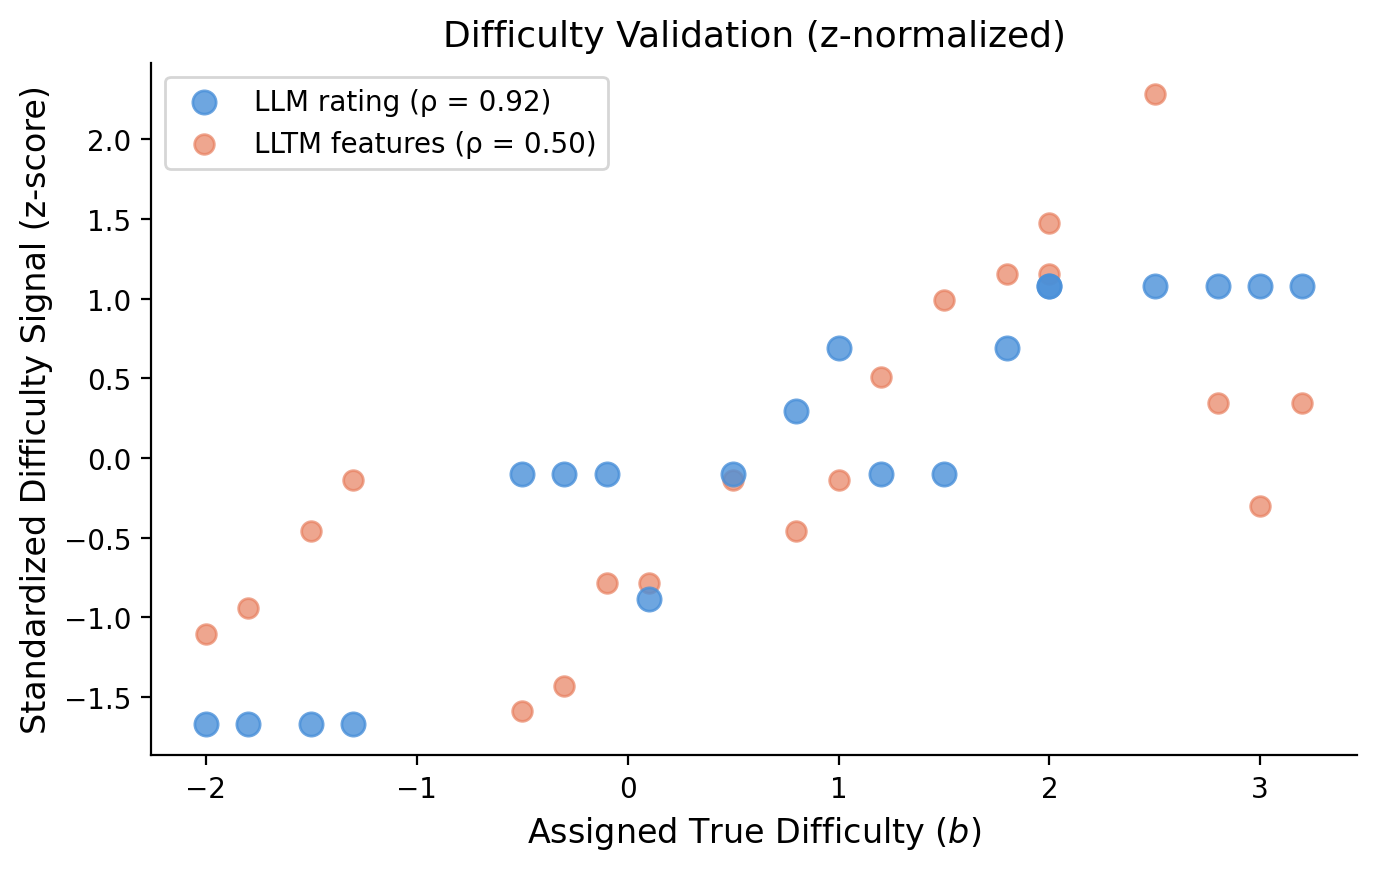
\includegraphics[width=0.65\linewidth]{figures/fig2_difficulty.png}
\caption{Difficulty validation (z-normalized). LLM ratings ($\rho = 0.919$) and LLTM features ($\rho = 0.50$) vs.\ author-assigned difficulty.}
\label{fig:diff}
\end{figure}

\FloatBarrier

\subsection{Equal-Budget Comparison}

\begin{table}[htbp]
\centering
\caption{Equal-budget results (4 chunks, 6 users, 3 judge repeats). Routing uses author-assigned difficulty validated by LLM ($\rho = 0.919$).}
\label{tab:main}
\small
\begin{tabular}{@{}lccr@{}}
\toprule
Strategy & Score (mean $\pm$ std) & Cohen's $d$ & Gap \\
\midrule
\textbf{PCR (ours)} & $\mathbf{6.06 \pm 1.39}$ & --- & --- \\
Corpus-prefix & $5.67 \pm 1.11$ & 0.31 & $-0.39$ \\
Fixed-random & $4.72 \pm 0.80$ & 1.18 & $-1.34$ \\
Difficulty-only & $3.67 \pm 2.36$ & 1.23 & $-2.39$ \\
\bottomrule
\end{tabular}
\end{table}

PCR achieves the highest score (Figure~\ref{fig:budget}).
The strongest result is vs.\ difficulty-only: $+2.39$, $d = 1.23$.
The advantage over corpus-prefix ($+0.39$, $d = 0.31$) is preliminary with 6~users.

\begin{figure}[htbp]
\centering
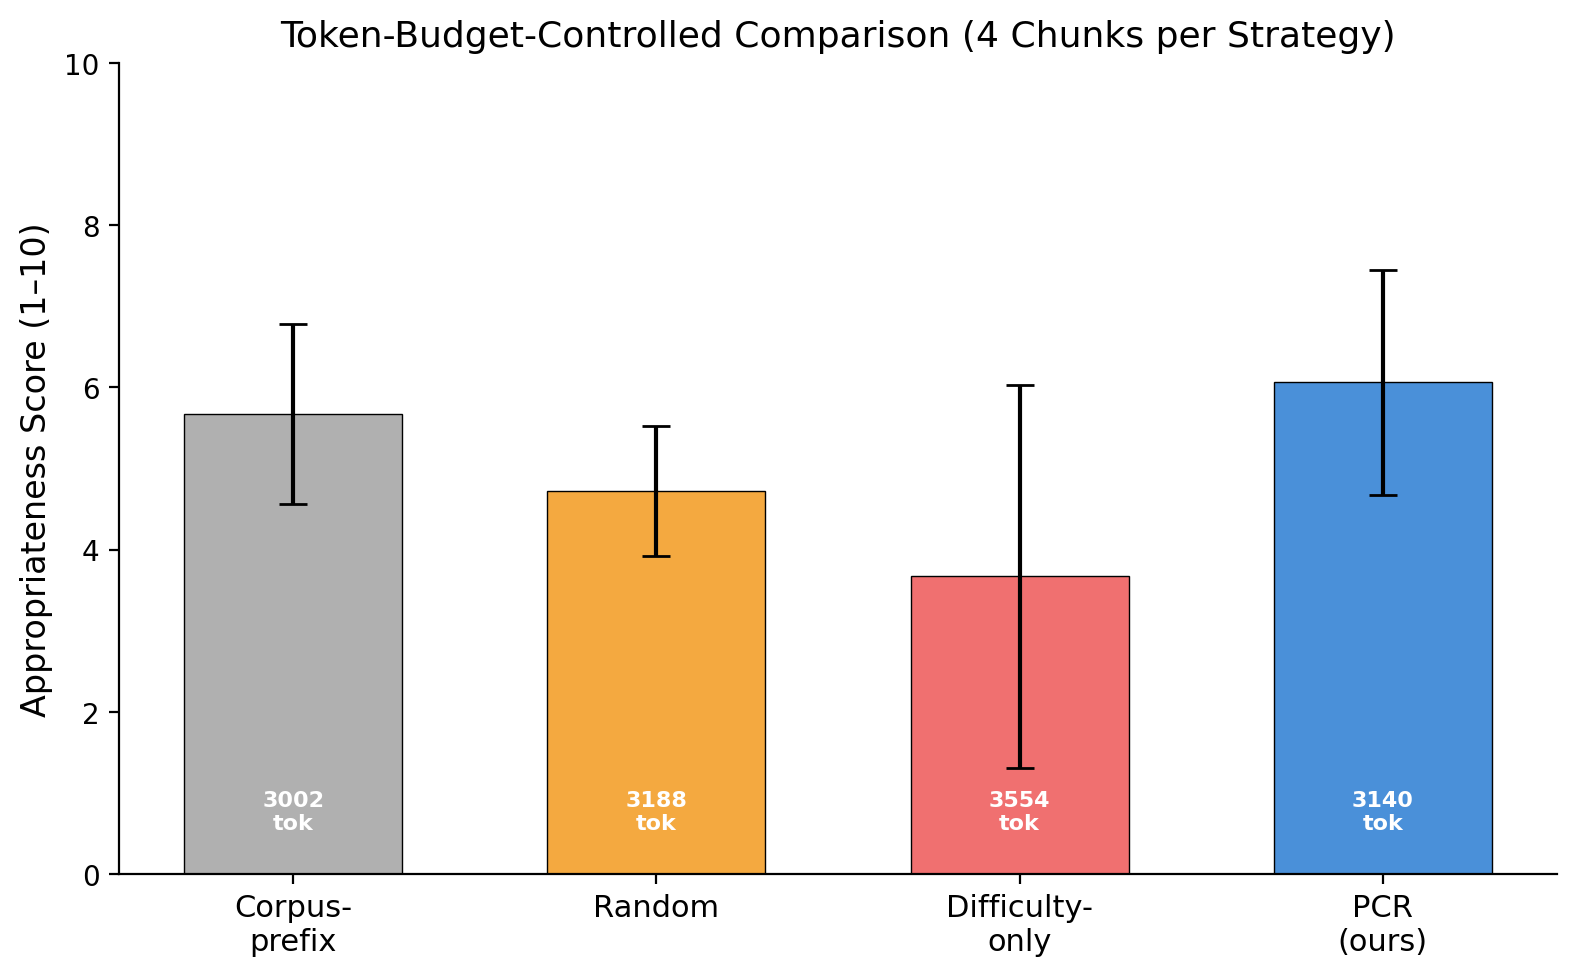
\includegraphics[width=0.65\linewidth]{figures/fig3_budget.png}
\caption{Equal-budget scores. Error bars: $\pm$1 std.}
\label{fig:budget}
\end{figure}

\FloatBarrier

\subsection{Pairwise Comparison}

\begin{table}[htbp]
\centering
\caption{Pairwise results (one-sided binomial). 18 = 6 users $\times$ 3 repeats.}
\label{tab:pair}
\small
\begin{tabular}{@{}lccc@{}}
\toprule
Comparison & PCR Wins & Eval $p$ & User $p$ \\
\midrule
PCR vs.\ Difficulty-only & 15/18 (83\%) & 0.004 & $\approx$0.109 \\
PCR vs.\ Fixed-random & 12/18 (67\%) & 0.119 & $\approx$0.344 \\
\bottomrule
\end{tabular}
\end{table}

\begin{figure}[htbp]
\centering
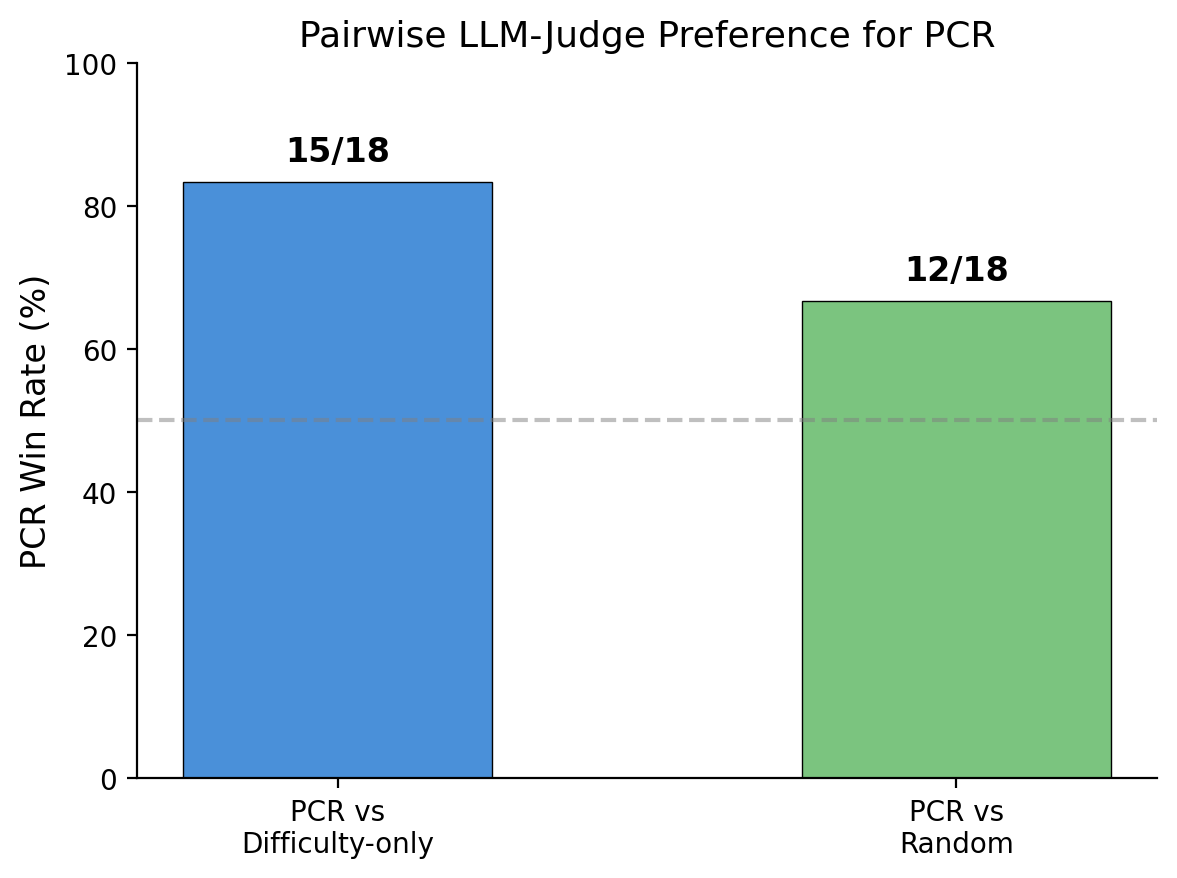
\includegraphics[width=0.50\linewidth]{figures/fig4_pairwise.png}
\caption{Pairwise LLM-judge preference. Dashed: chance.}
\label{fig:pair}
\end{figure}

\FloatBarrier

\subsection{Per-Ability Content Selection}

Figure~\ref{fig:route} shows PCR selections per user.
A $\theta = -2$ student gets elementary passages; a $\theta = +3$ researcher gets graduate passages.

\begin{figure}[htbp]
\centering
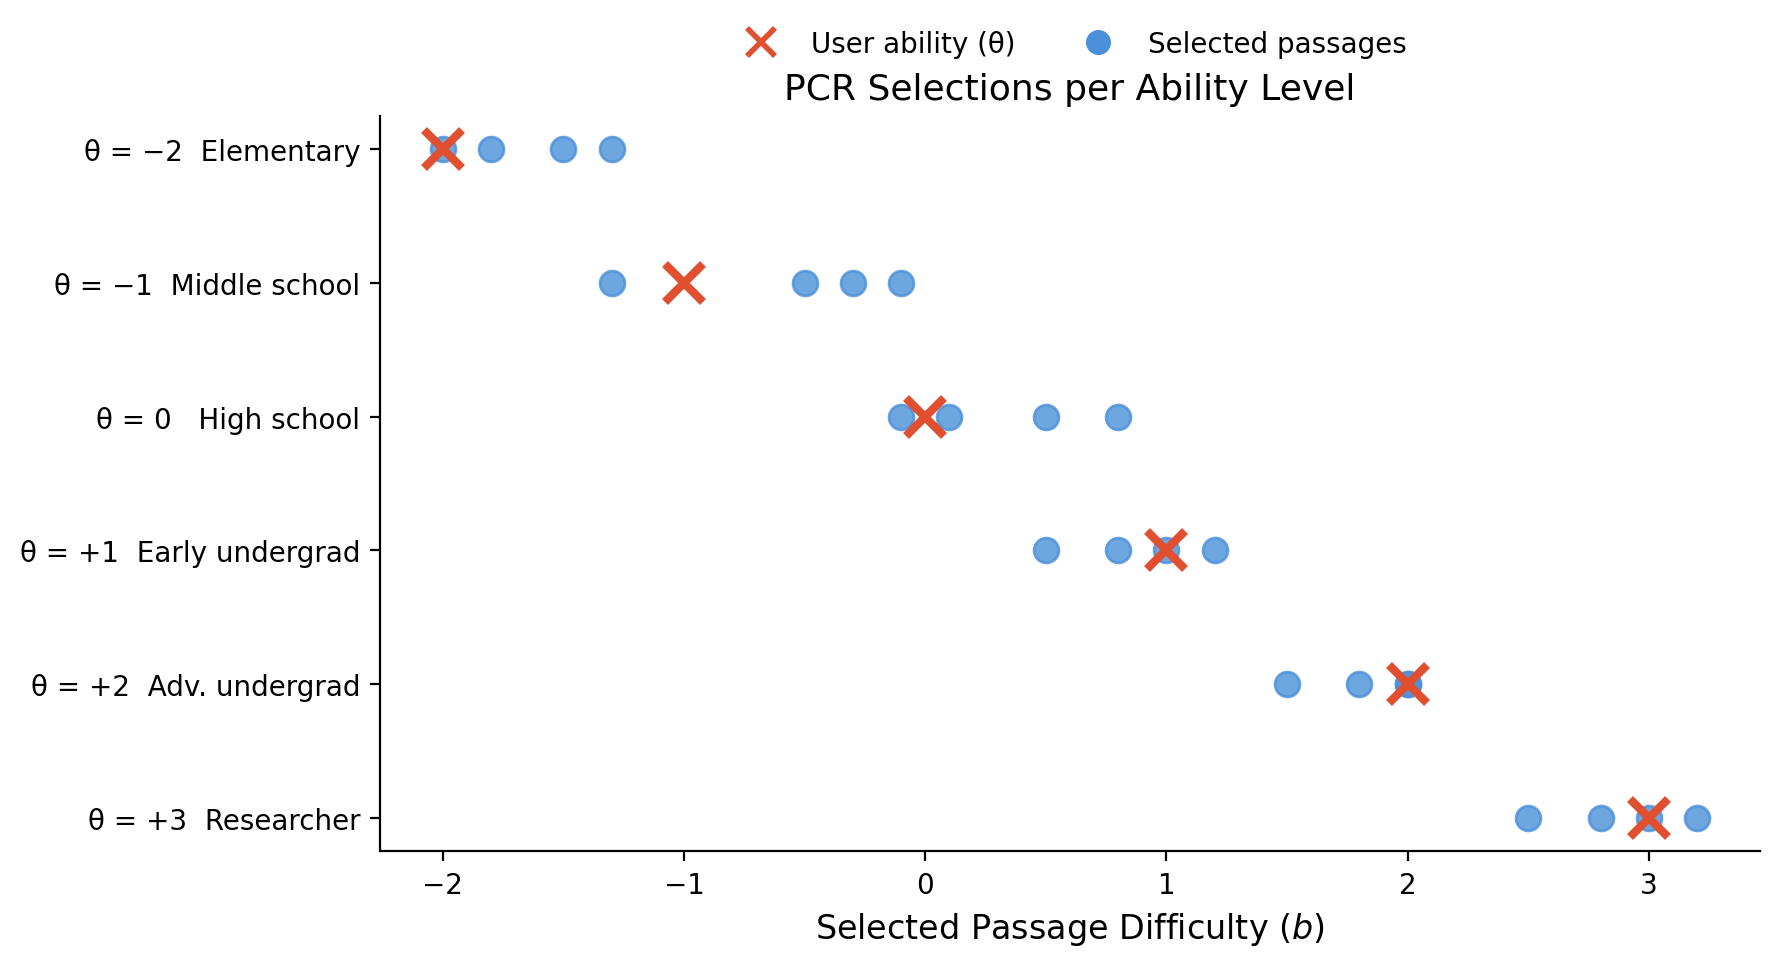
\includegraphics[width=0.72\linewidth]{figures/fig5_routing.png}
\caption{PCR selections per ability level.}
\label{fig:route}
\end{figure}

\FloatBarrier

\subsection{Simulation: Scaling with Diversity}

In simulation (50 users, 200 items, 30\% budget, 10 seeds), PCR's advantage over uniform random selection grows from $1.49\times$ to $3.15\times$ as difficulty diversity increases (Figure~\ref{fig:scale}).

\begin{figure}[htbp]
\centering
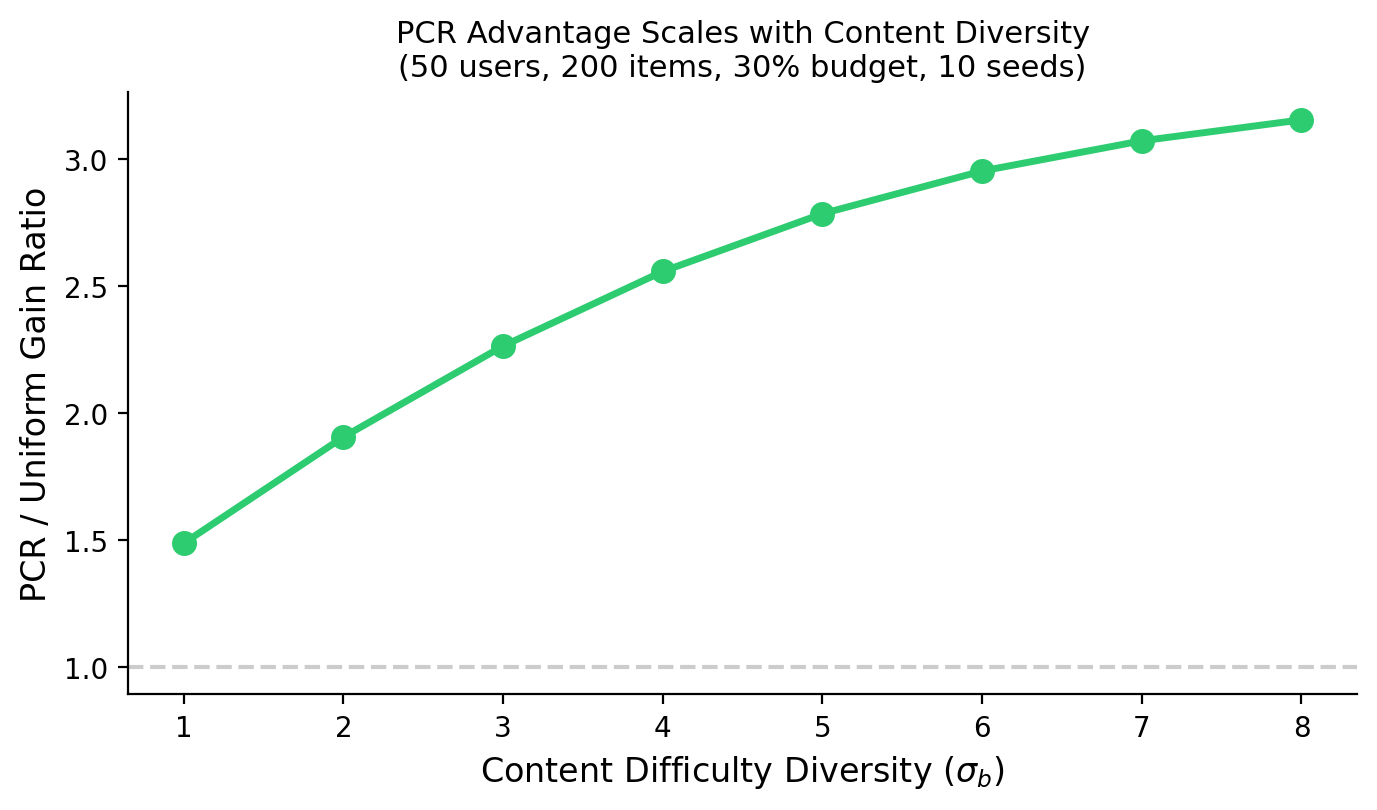
\includegraphics[width=0.58\linewidth]{figures/fig6_scaling.png}
\caption{PCR advantage grows with difficulty diversity.}
\label{fig:scale}
\end{figure}

\FloatBarrier

\section{Discussion}

\paragraph{Why difficulty-only fails.}
It selects the same hardest passages for all users.
Its variance ($\pm 2.36$) reflects success for experts but failure for novices, confirming that $\theta$-conditioning is essential~\citep{kang2026efsl}.

\paragraph{Difficulty source.}
The reported results use author-assigned difficulty, which provides an upper bound on PCR performance.
In deployment, difficulty can come from LLM rating ($\rho = 0.919$, requires API calls) or LLTM features ($\rho = 0.50$, zero cost).
Future work should evaluate PCR end-to-end with LLTM-estimated difficulty to measure the impact of noisier difficulty estimates on routing quality.

\paragraph{Connection to ZPD Detector.}
Yang et al.~\citep{yang2026zpd} concurrently proposed IRT-based capability--difficulty matching for training data selection.
PCR differs: (1)~ability represents the \emph{user}, not the model; (2)~selection is at \emph{inference} time; (3)~LLTM provides interpretable feature decomposition.

\paragraph{Connection to RAG.}
RAG selects by relevance; PCR by frontier value.
These are orthogonal; a production system retrieves by relevance, then reranks by $\mathcal{F}$.

\paragraph{Limitations.}
(1)~20 passages, author-assigned difficulty.
(2)~LLM-judge biases~\citep{zheng2023judging}.
(3)~Six users; limited user-level power.
(4)~$\theta$ assumed known.
(5)~LLTM features weak ($\rho = 0.50$); trained embeddings would improve.
(6)~Routing used author-assigned difficulty, not LLTM estimates; end-to-end LLTM routing is future work.
(7)~Corpus-prefix is not truly uniform.
(8)~Fixed-random baseline uses a single seed; a multi-seed average would be a stronger comparator.

\section{Related Work}

\textbf{IRT in AI.}
Rodriguez et al.~\citep{rodriguez2021evaluation}, Zhou et al.~\citep{zhou2026psnirt}, Kang~\citep{kang2026efsl}.
\textbf{IRT routing.}
Song et al.~\citep{song2025irtrouter}: between-LLM routing (ACL 2025).
\textbf{ZPD for selection.}
Yang et al.~\citep{yang2026zpd}: training data selection.
PCR: user-facing inference-time routing.
\textbf{Personalization.}
Nguyen et al.~\citep{nguyen2026pragedu}: grade-level RAG.
Wang et al.~\citep{wang2025claf}: cognitive-level output adaptation.
\textbf{RAG.}
Peng et al.~\citep{peng2026adagres}, Allu et al.~\citep{allu2026wrac}.

\section{Conclusion}

PCR strongly outperforms difficulty-only selection ($d = 1.23$, $p = 0.004$, 83\% pairwise) and trends above other baselines when routing on validated difficulty labels.
LLTM provides a weaker but API-free difficulty proxy ($\rho = 0.50$), offering a scalable path.
Future work: end-to-end LLTM-routed PCR, PCR as a RAG reranker, human judges, and stronger baselines.

\paragraph{Reproducibility.}
The supplementary archive contains:
\begin{itemize}[nosep,leftmargin=1.5em]
  \item \LaTeX{} source and all six figures;
  \item 20-passage corpus with full text and LLTM features;
  \item user profiles and exact prompts for all four phases;
  \item runnable experiment script (\texttt{src/run\_experiment.py});
  \item LLTM feature extraction (\texttt{src/extract\_lltm\_features.py});
  \item simulation figure code for Figures~1 and~6;
  \item reported-run summary statistics.
\end{itemize}
Figures~2--5 are static images from the original run.
Raw generations, judge votes, and cached API responses will be released in the accompanying repository.

\bibliographystyle{plainnat}
\begin{thebibliography}{16}
\bibitem[Allu et al.(2026)]{allu2026wrac} Allu, U., et al. W-RAC for Efficient RAG Systems. \emph{arXiv:2604.04936}, 2026.
\bibitem[Fischer(1973)]{fischer1973lltm} Fischer, G.\,H. The linear logistic test model as an instrument in educational research. \emph{Acta Psychologica}, 37:359--374, 1973.
\bibitem[Kang(2026)]{kang2026efsl} Kang, J.\,M. The Scaling Law of Evaluation Failure. \emph{arXiv:2605.11205}, 2026.
\bibitem[Laitenberger et al.(2026)]{laitenberger2025gateskip} Laitenberger, F., et al. What Layers When: Learning to Skip Compute in LLMs with Residual Gates. In \emph{ICLR}, 2026.
\bibitem[Lord and Novick(1968)]{lord1968statistical} Lord, F.\,M. and Novick, M.\,R. \emph{Statistical Theories of Mental Test Scores}. Addison-Wesley, 1968.
\bibitem[Nguyen et al.(2026)]{nguyen2026pragedu} Nguyen, V.\,D., et al. Towards Personalized AI Education: Context-Aware RAG with Grade-Level LLM Adaptation. \emph{Comp.\ Appl.\ Eng.\ Educ.}, 34:e70153, 2026.
\bibitem[Peng et al.(2026)]{peng2026adagres} Peng, C., et al. AdaGReS: Adaptive Greedy Context Selection for Token-Budgeted RAG. \emph{arXiv:2512.25052}, 2026.
\bibitem[Raposo et al.(2024)]{raposo2024mod} Raposo, D., et al. Mixture-of-Depths. \emph{arXiv:2404.02258}, 2024.
\bibitem[Rodriguez et al.(2021)]{rodriguez2021evaluation} Rodriguez, P., et al. Evaluation Examples Are Not Equally Informative. In \emph{ACL-IJCNLP}, pp.~4486--4503, 2021.
\bibitem[Song et al.(2025)]{song2025irtrouter} Song, W., et al. IRT-Router: Multi-LLM Routing via IRT. In \emph{ACL}, pp.~15629--15644, 2025.
\bibitem[Vygotsky(1978)]{vygotsky1978mind} Vygotsky, L.\,S. \emph{Mind in Society}. Harvard University Press, 1978.
\bibitem[Wang et al.(2025)]{wang2025claf} Wang, Q., et al. Cognitive-Level Adaptive Generation via CLAF. In \emph{Findings of EMNLP}, 2025.
\bibitem[Yang et al.(2026)]{yang2026zpd} Yang, B., et al. ZPD Detector: Data Selection via Capability--Difficulty Alignment for LLMs. \emph{arXiv:2601.10986}, 2026.
\bibitem[Zheng et al.(2023)]{zheng2023judging} Zheng, L., et al. Judging LLM-as-a-Judge with MT-Bench and Chatbot Arena. In \emph{NeurIPS}, 2023.
\bibitem[Zhou et al.(2026)]{zhou2026psnirt} Zhou, H., et al. Lost in Benchmarks? LLM Benchmarking with IRT. In \emph{AAAI}, 40(41):35085--35093, 2026.
\end{thebibliography}

\end{document}
